% !TeX root = ./0_slides.tex

\section{DFF logic path under BBI}
\begin{frame}{DFF schematic: CORE65GPSVT\_HS65\_GS\_DFPQX4}
	\centering
	\vspace{2mm}
	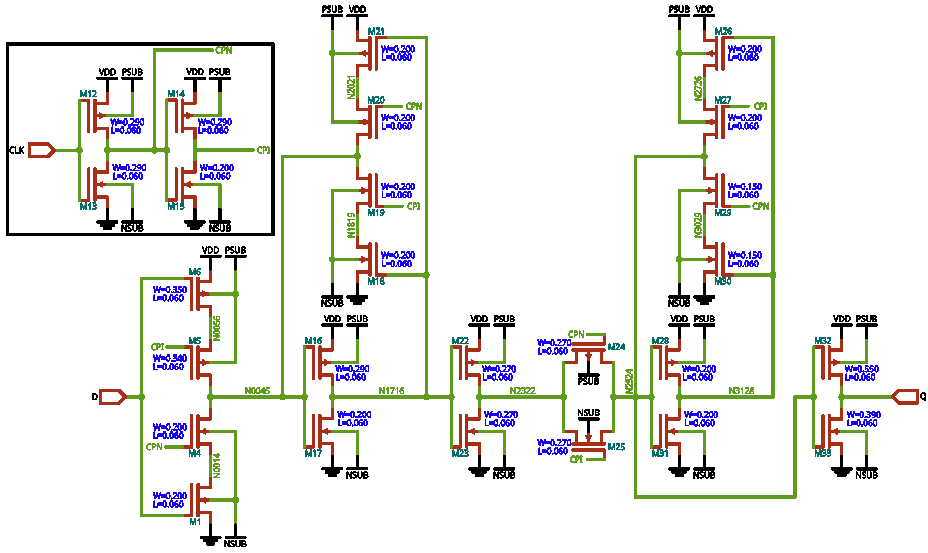
\includegraphics[width=\textwidth]{./figures/CORE65GPSVT_HS65_GS_DFPQX4.pdf}
\end{frame}

\begin{frame}{Inverters and buffers schematics}
	\centering
	\vspace{5mm}
	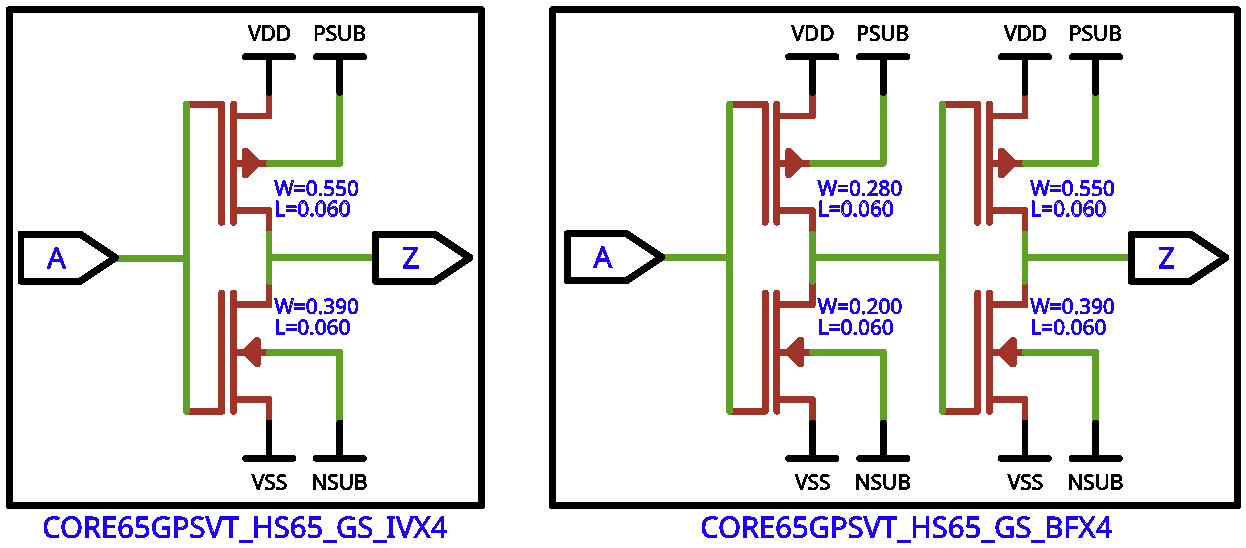
\includegraphics[width=\textwidth]{./figures/IVX_BUFF_X4.pdf}
\end{frame}

\begin{frame}{Simulated symbolic netlist}
	\centering
	\vspace{15mm}
    \begin{textblock*}{145mm}(0mm, 30mm)
		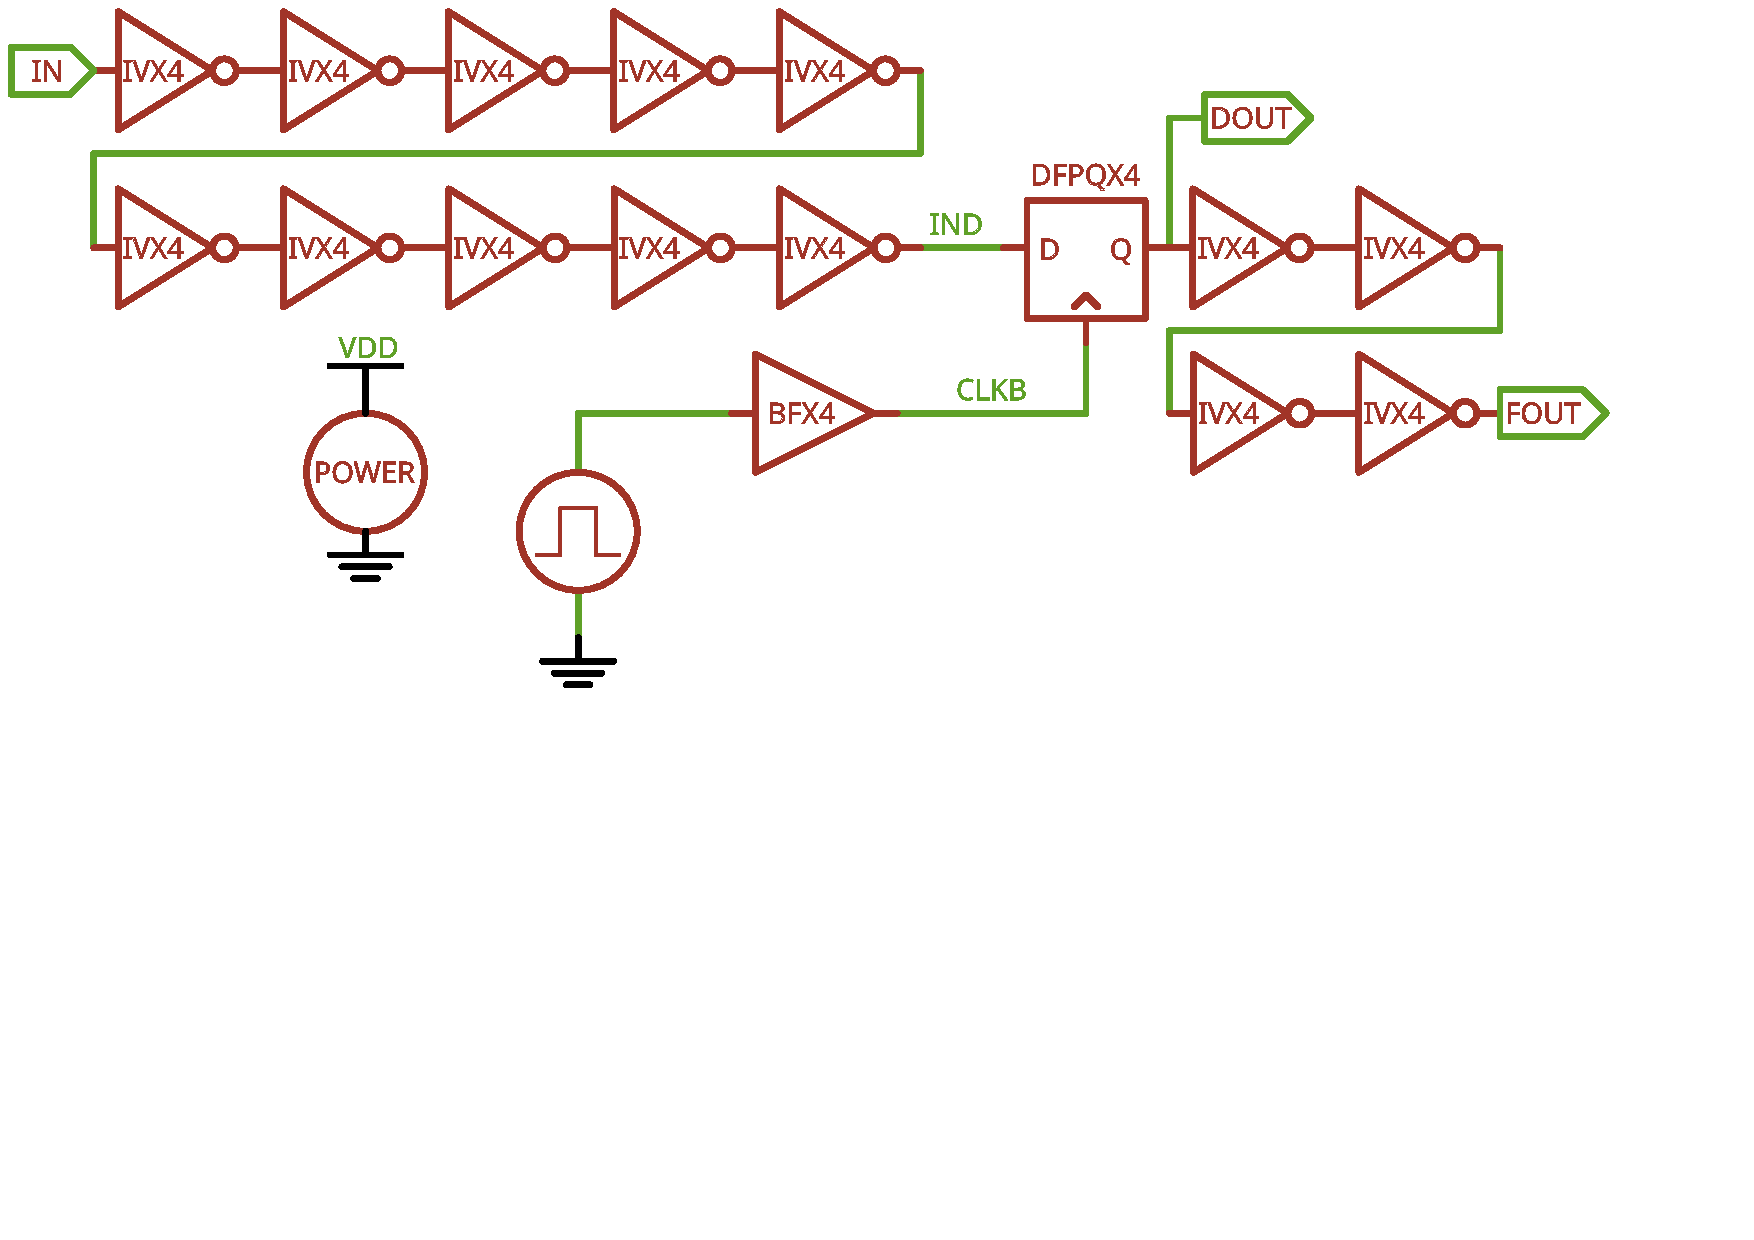
\includegraphics[width=1.0\textwidth]{./figures/dff_ivx_chain.pdf}
	\end{textblock*}
\end{frame}

\begin{frame}{DFF simulation: IDLE NORMALLY HIGH}
	\centering
	\vspace{2mm}
	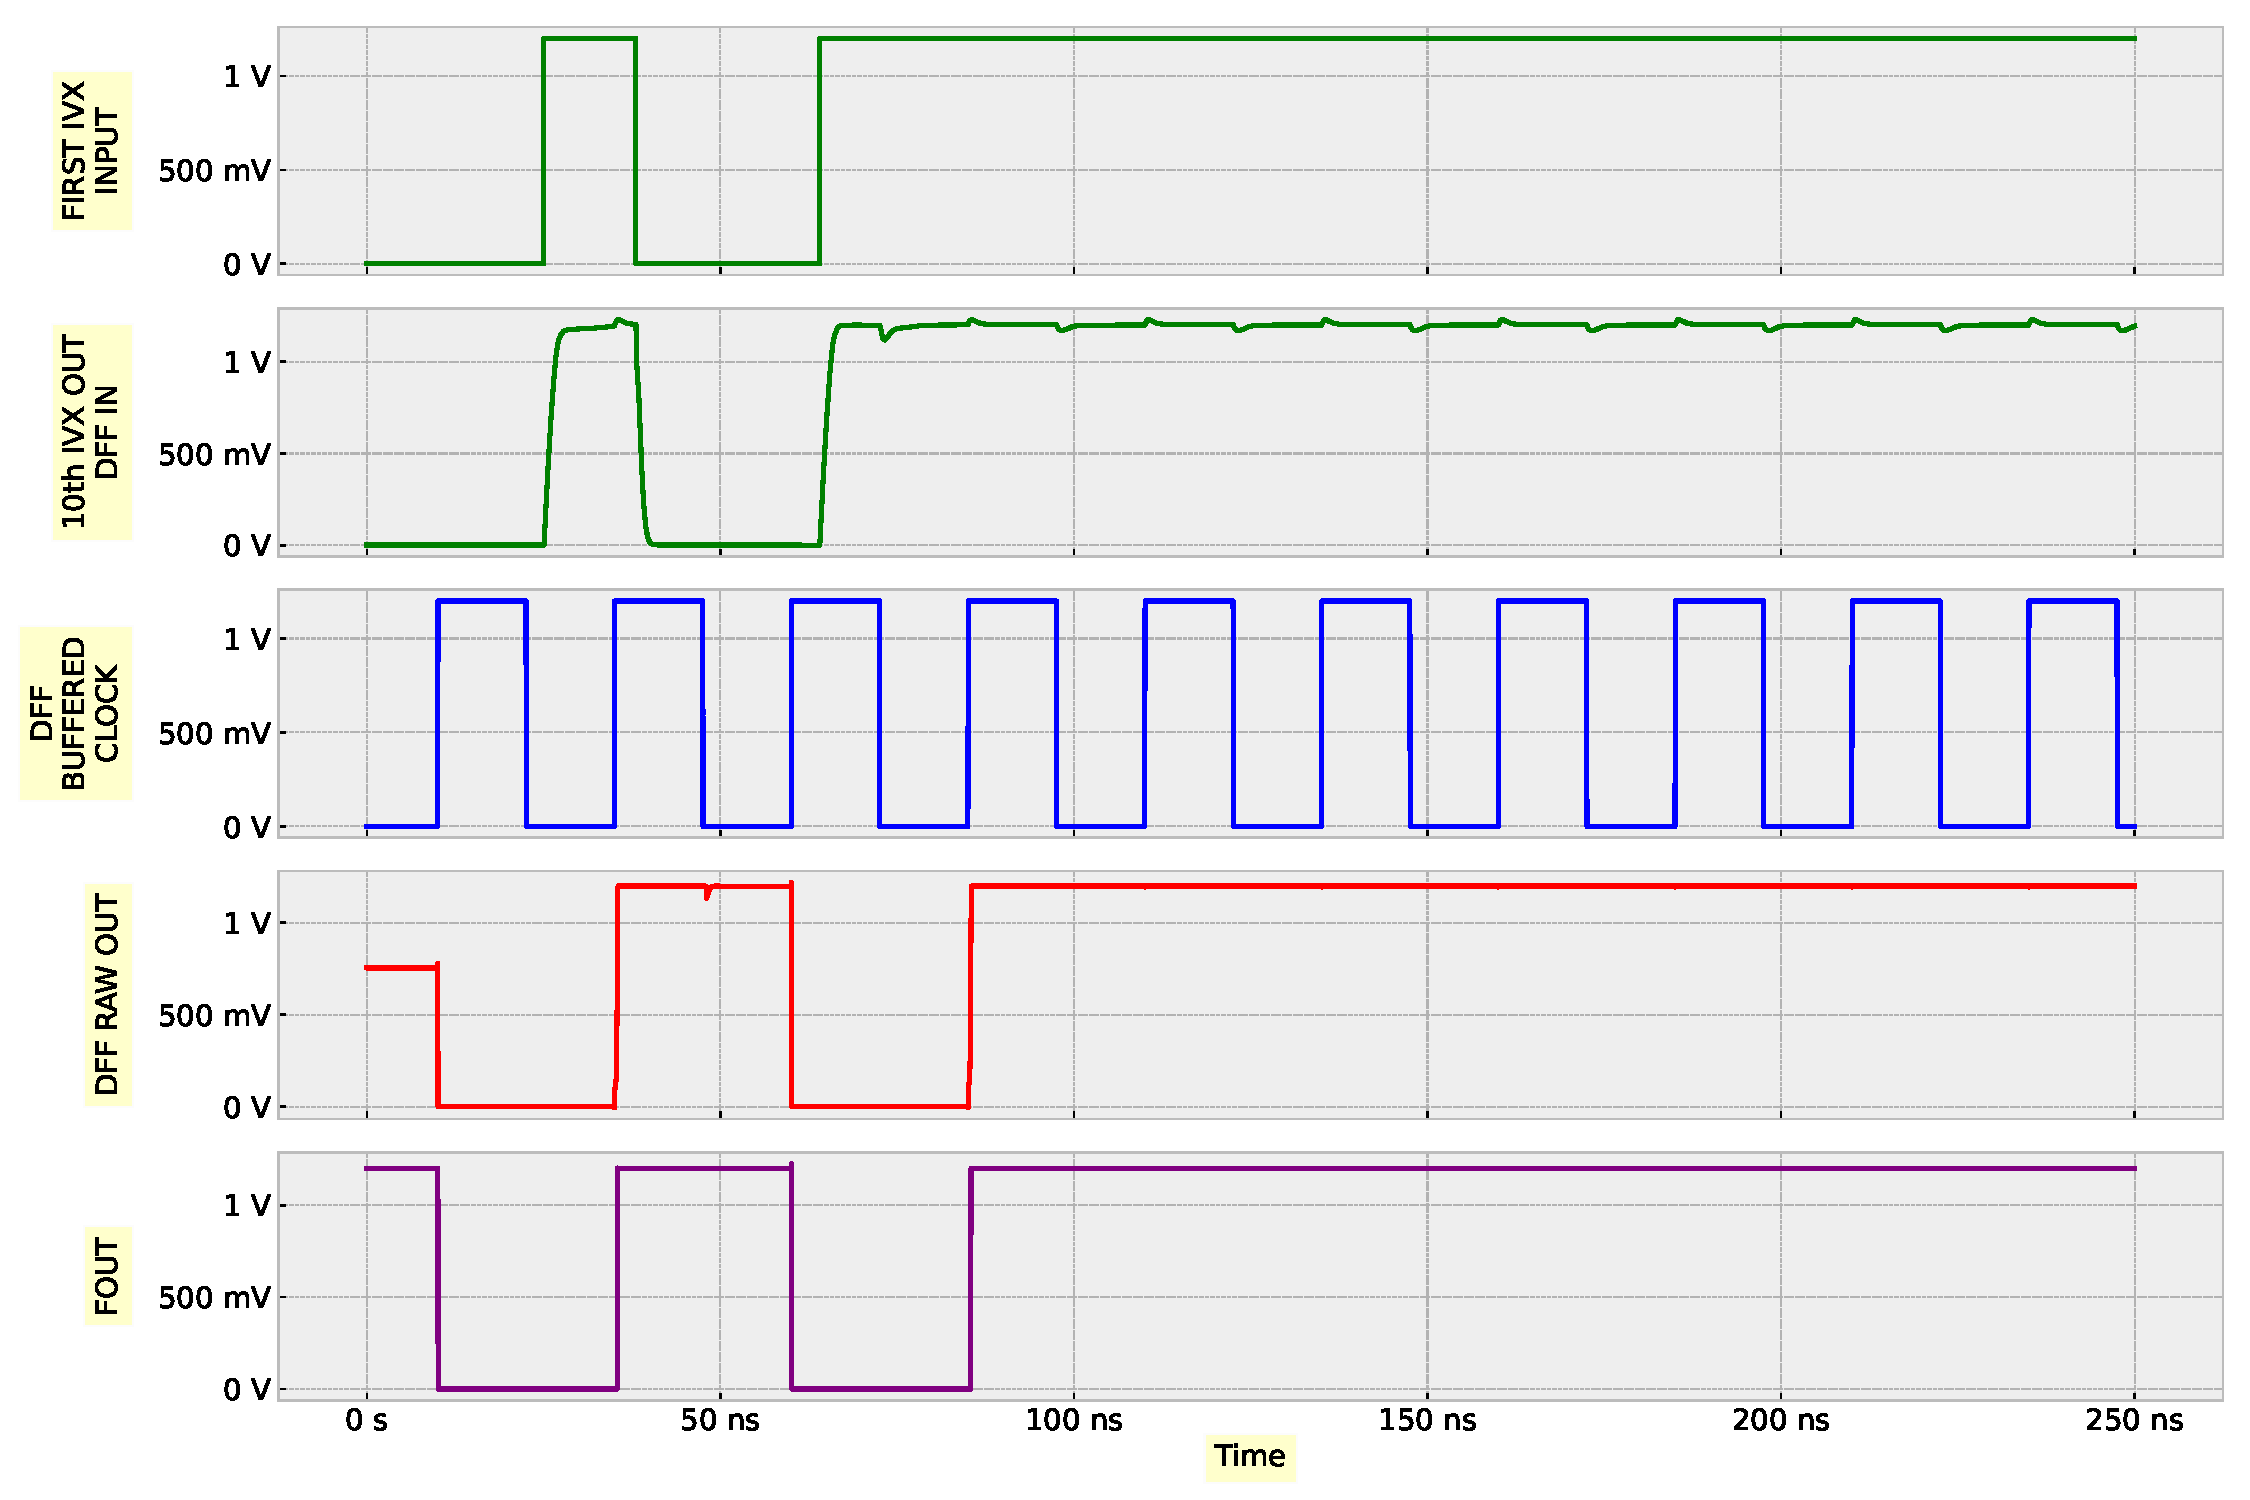
\includegraphics[width=\textwidth]{./figures/DFPX4_idle_nLow.pdf}
\end{frame}

\begin{frame}{DFF simulation: BBI NORMALLY HIGH}
	\centering
	\vspace{2mm}
	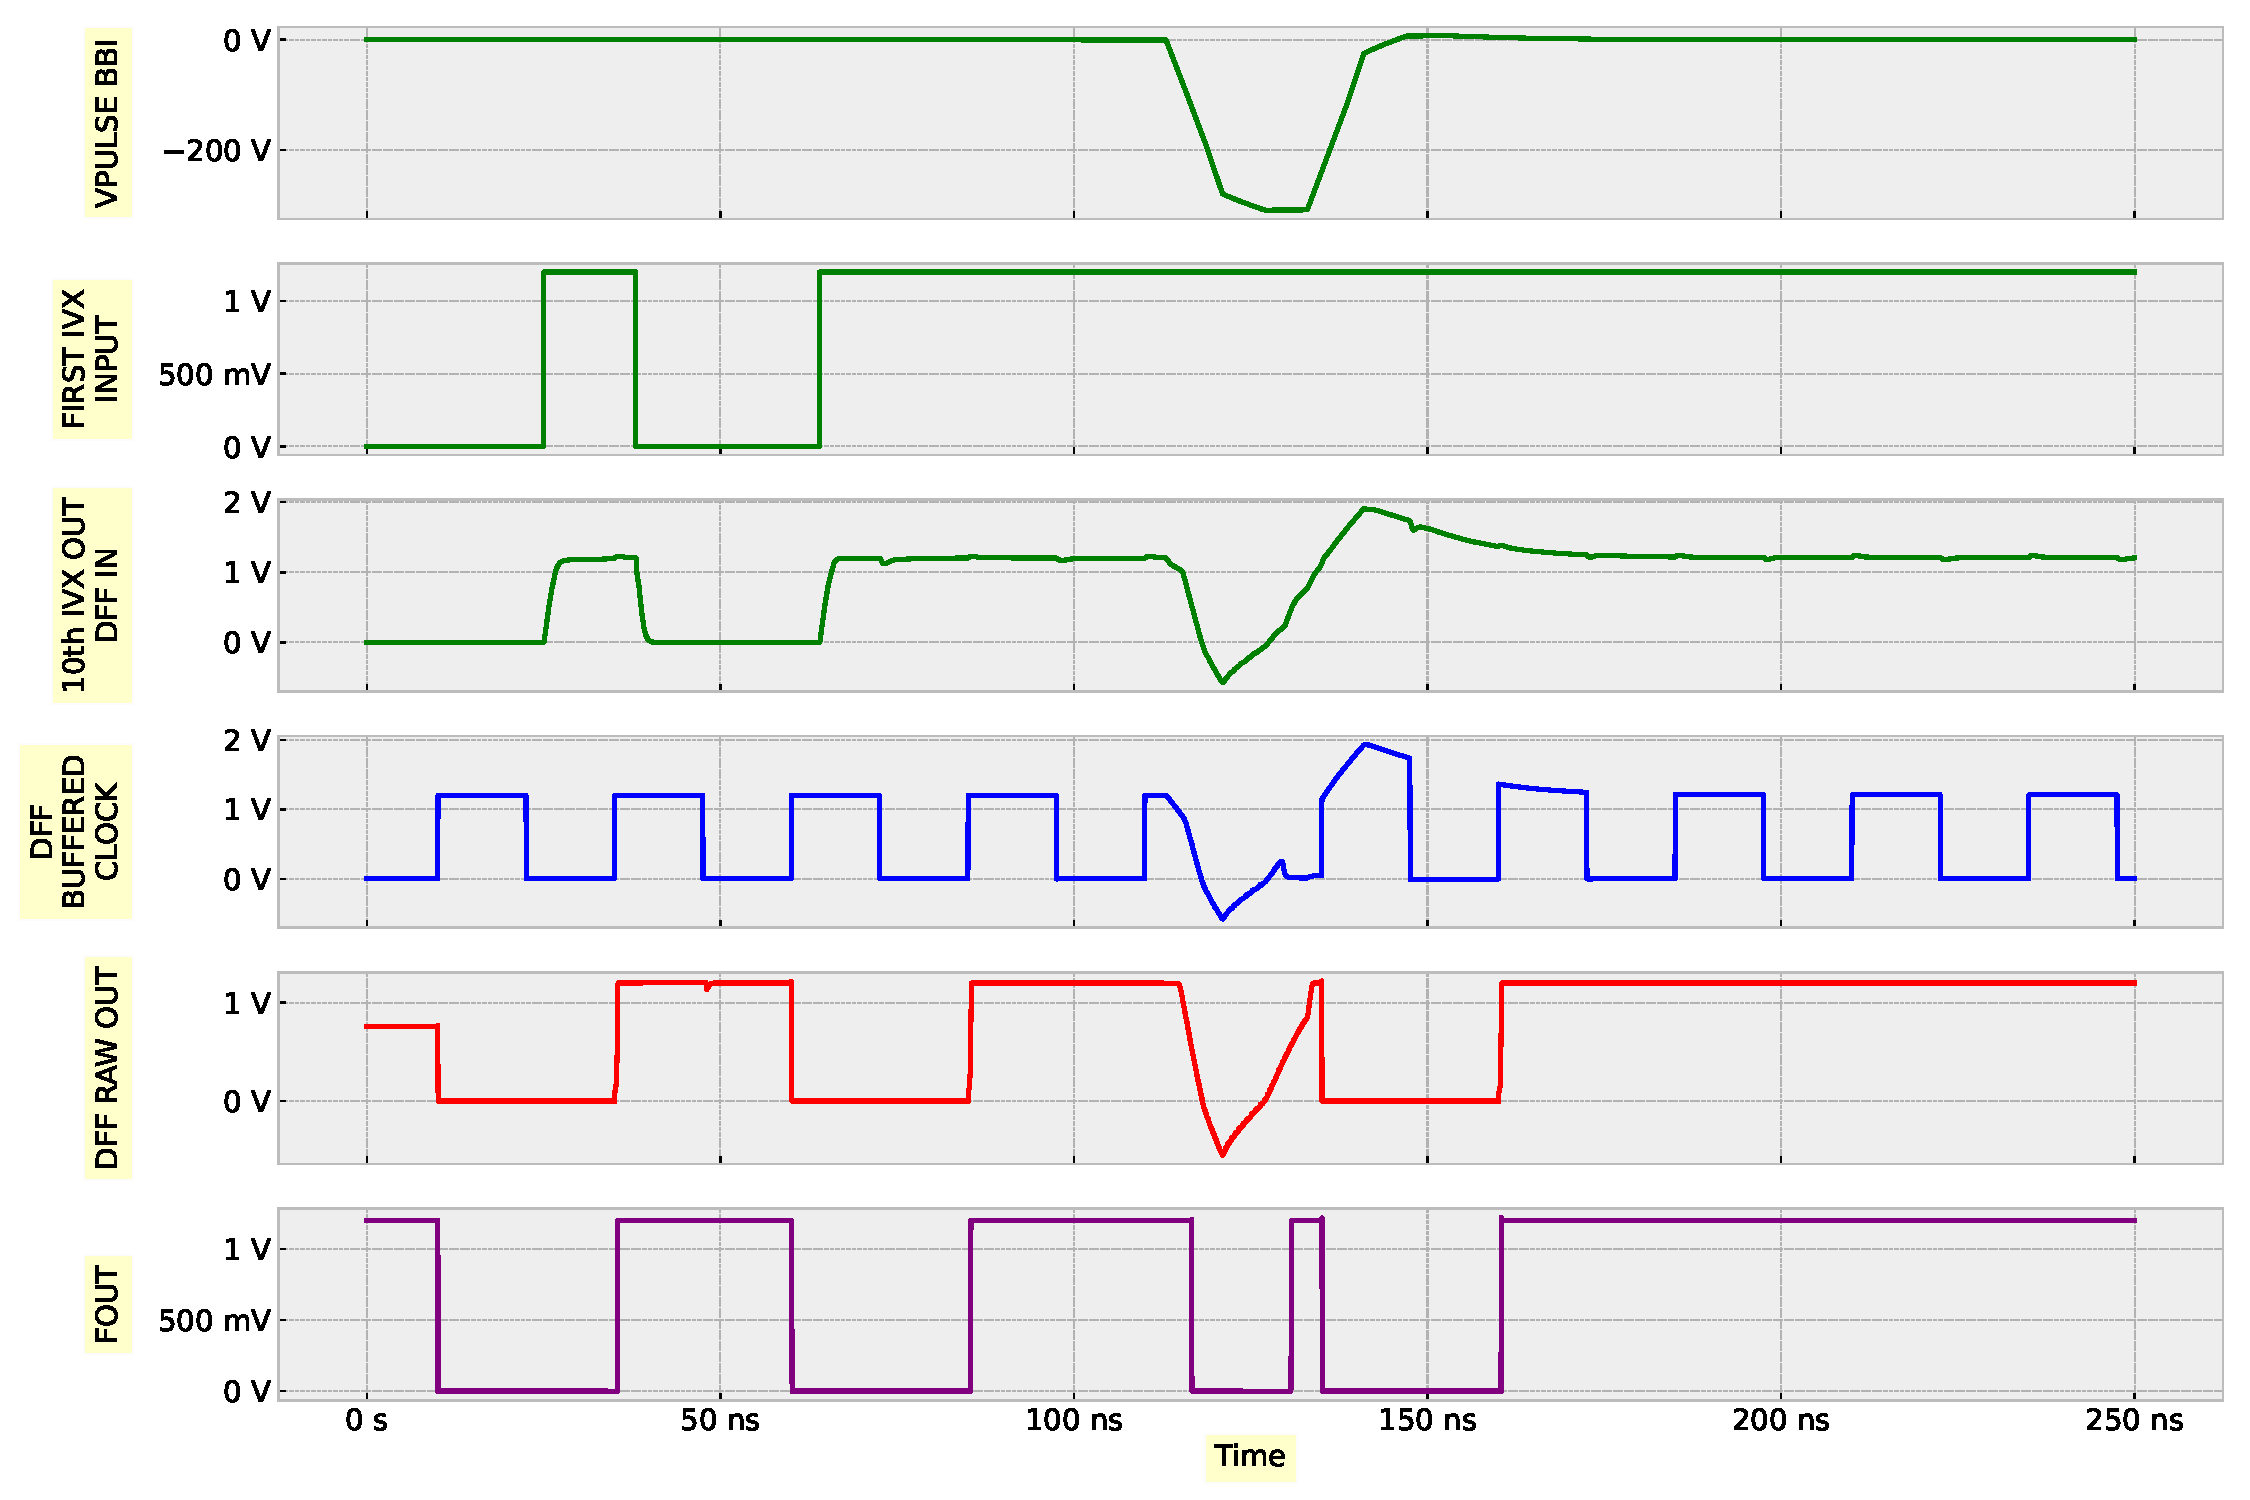
\includegraphics[width=\textwidth]{./figures/DFPX4_bbi_nLow.pdf}
\end{frame}

\begin{frame}{DFF simulation: IDLE NORMALLY LOW}
	\centering
	\vspace{2mm}
	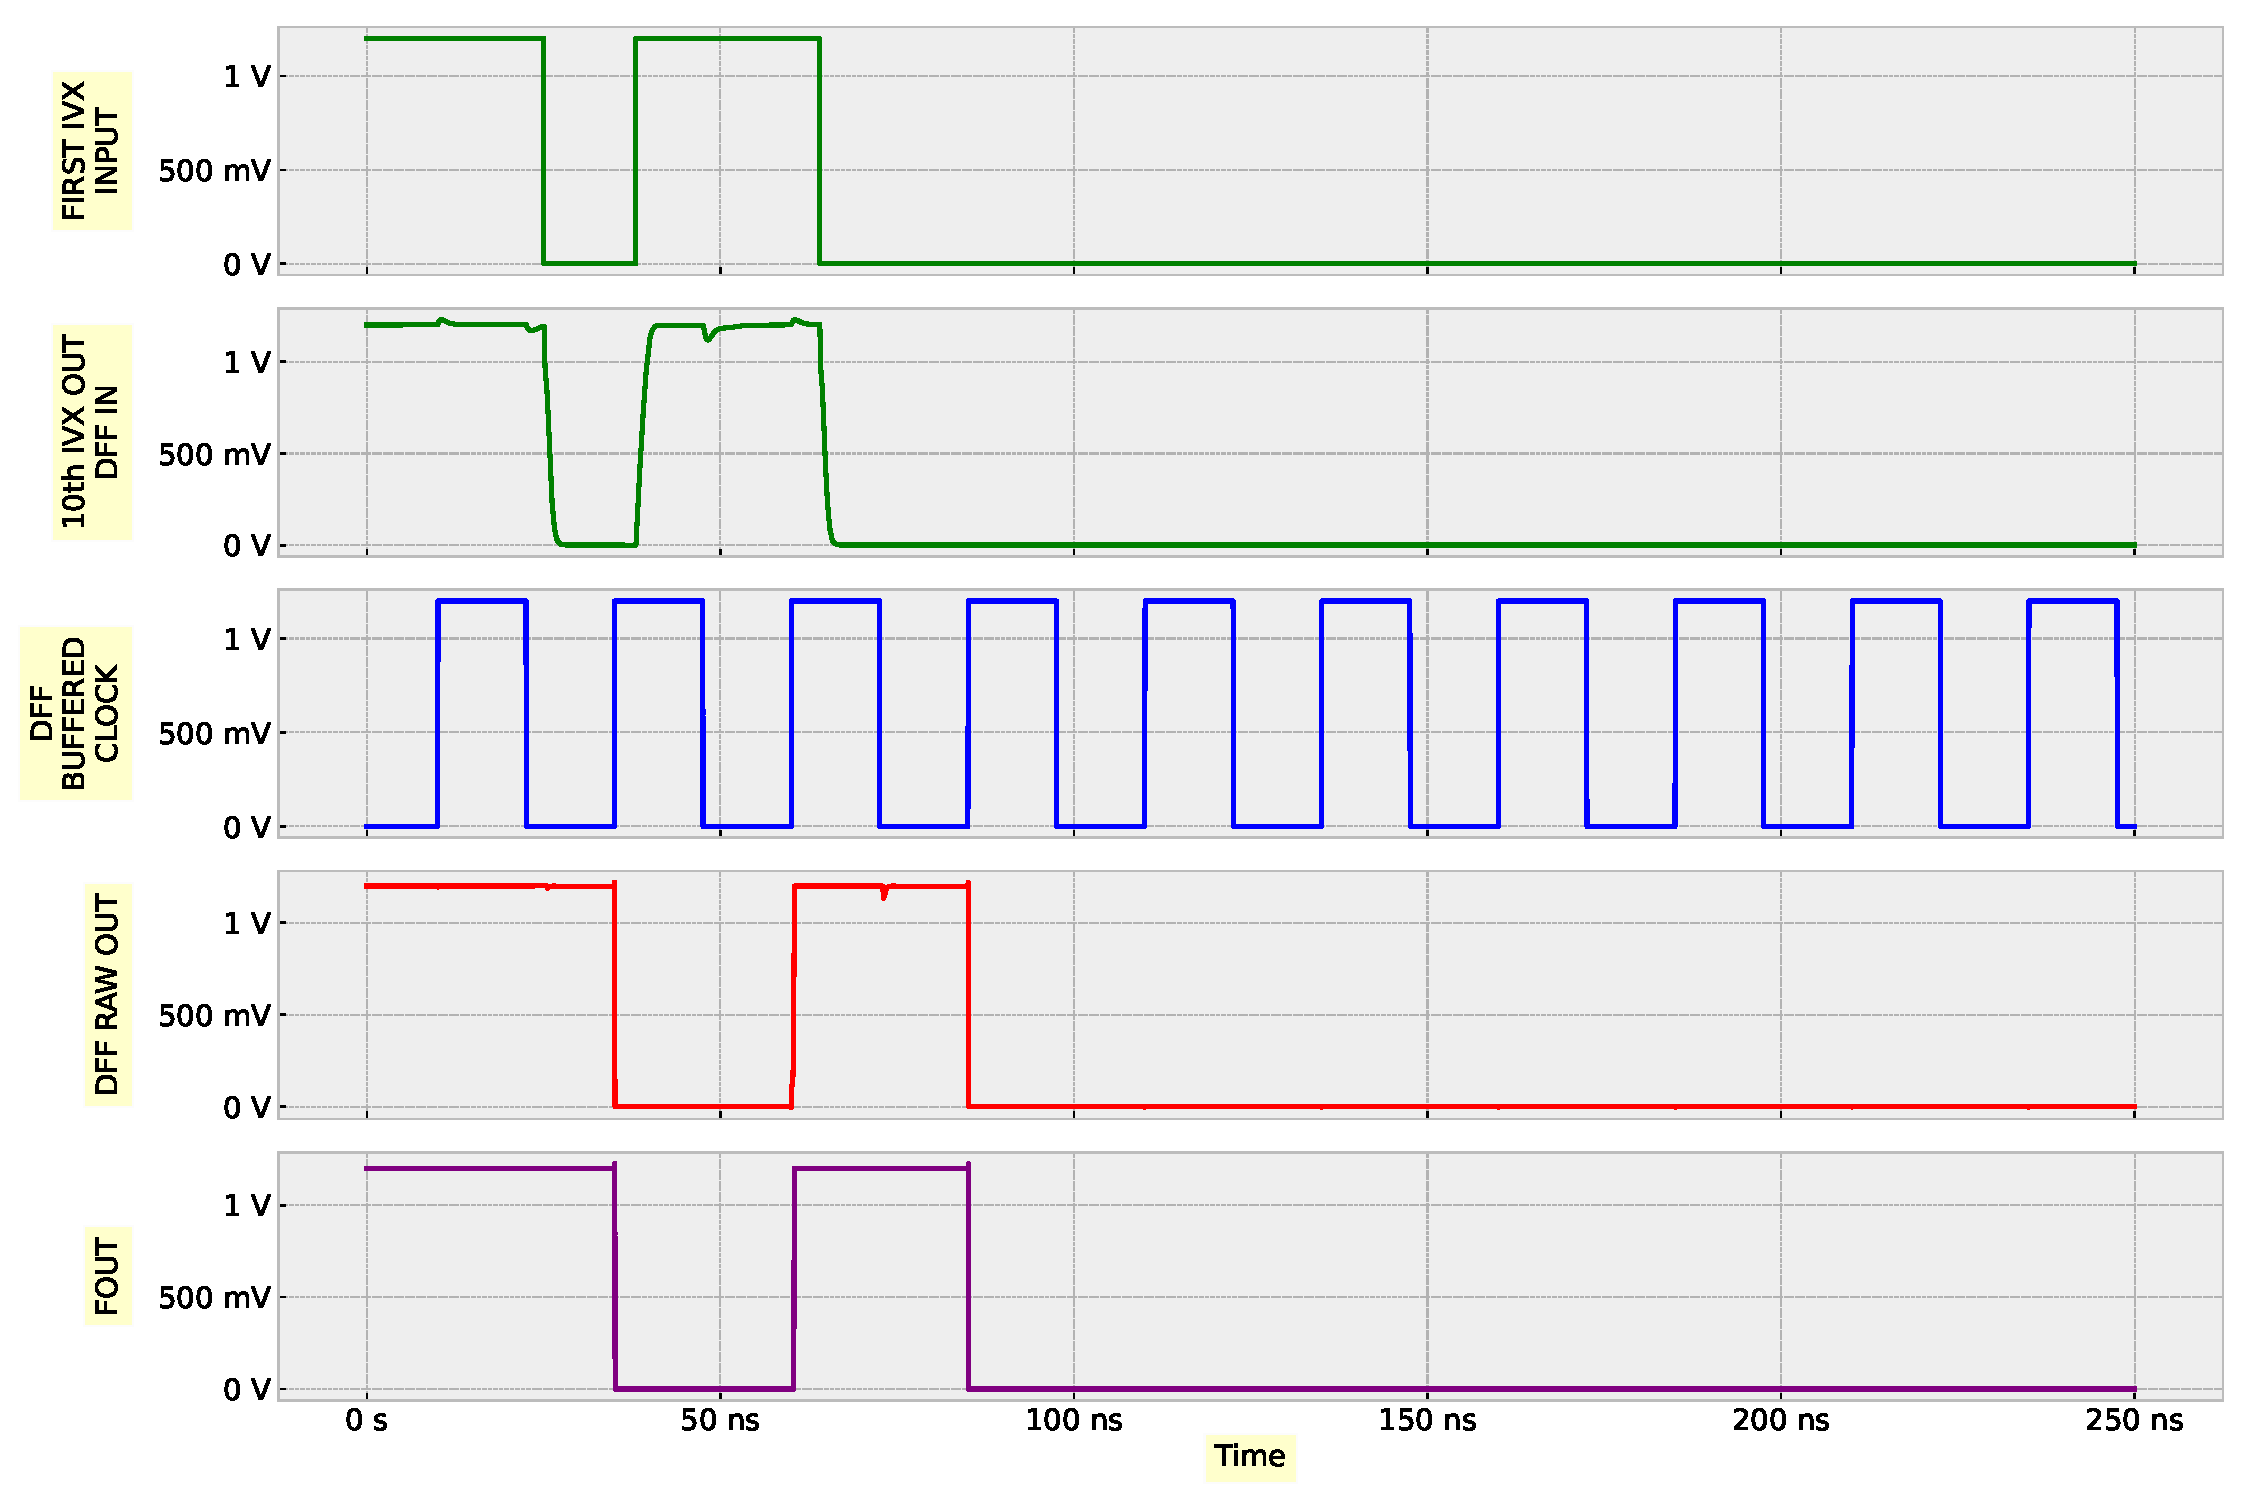
\includegraphics[width=\textwidth]{./figures/DFPX4_idle_nHigh.pdf}
\end{frame}

\begin{frame}{DFF simulation: BBI NORMALLY LOW}
	\centering
	\vspace{2mm}
	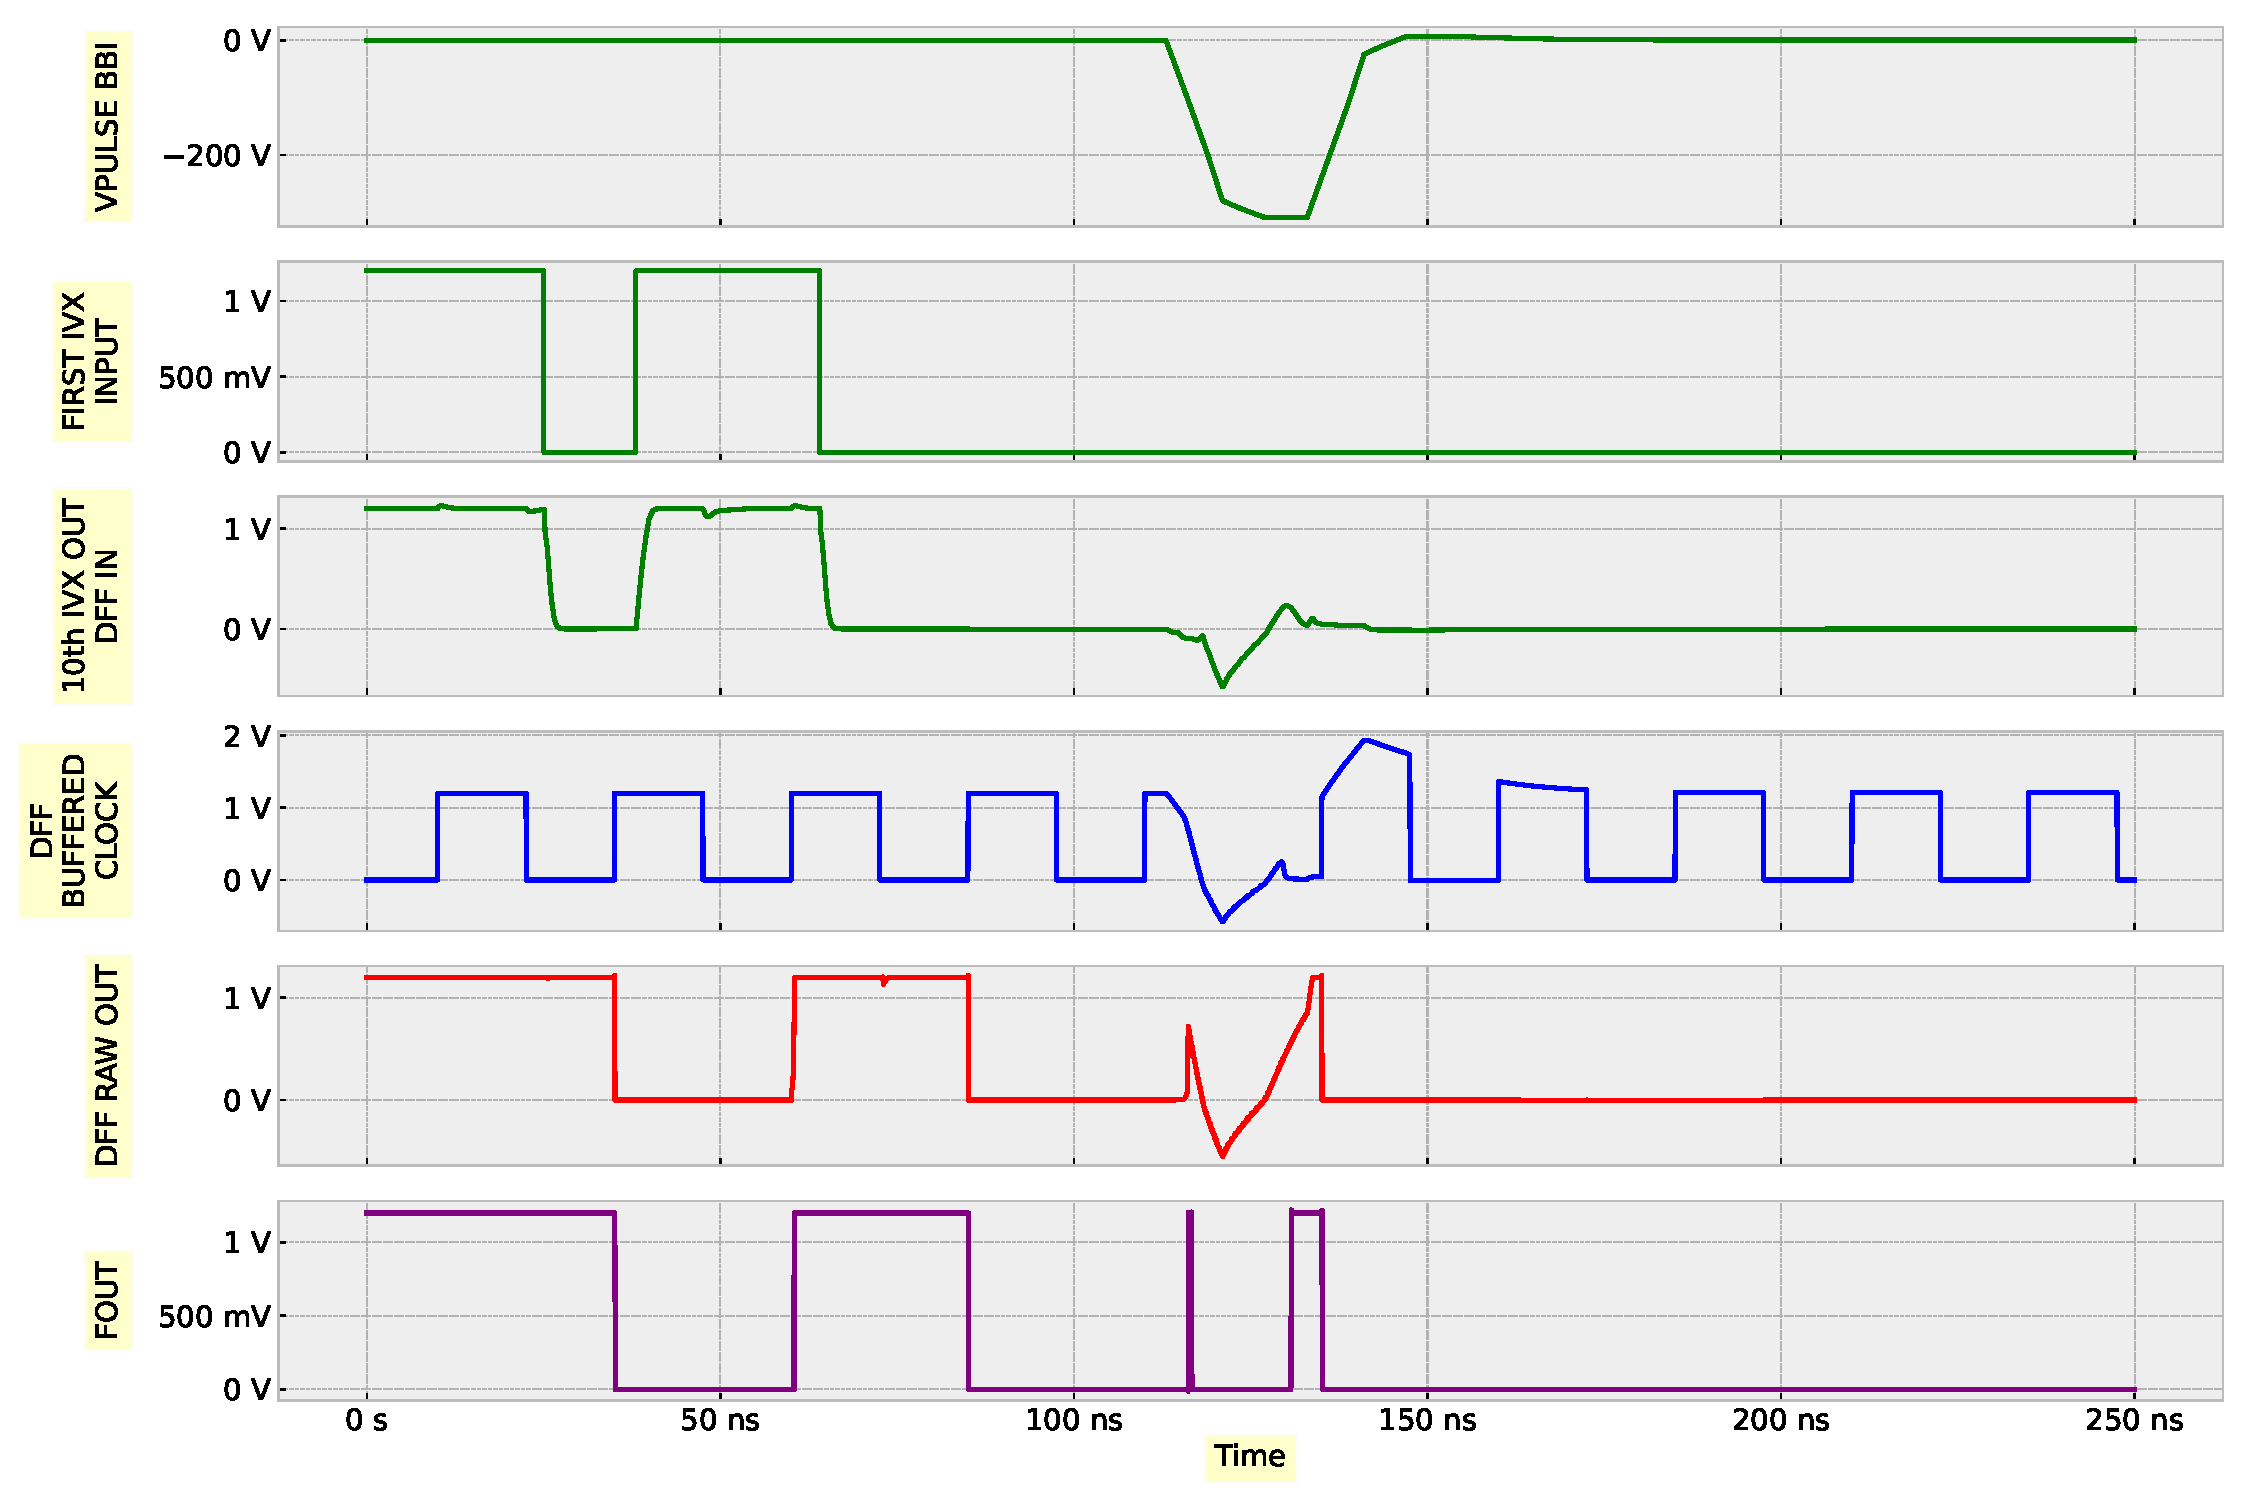
\includegraphics[width=\textwidth]{./figures/DFPX4_bbi_nHigh.pdf}
\end{frame}

\begin{frame}{BLANK FRAME}
	NO CONTENT
\end{frame}
